\chapter{Testy systemu (AK i JC)}
\label{cha:tests}

% setup
\graphicspath{{6_tests/static/}}

% content
Niniejszy rozdział stanowi szczegółowy raport z~przeprowadzanych w~środowisku docelowym testów systemu GGSS. Został on podzielony na trzy części, opisujące różne rodzaje przeprowadzanych przez autorów sprawdzeń. Pierwsza z~nich przybliża informacje dotyczące przeprowadzanych w~sposób cykliczny testów - nacisk położony został tutaj przede wszystkim na opis powtarzanej w~każdej iteracji procedury pozwalającej zweryfikować poprawność działania systemu. Druga część stanowi opis sprawdzeń wykonywanych w~czasie mającej miejsce w~lipcu 2021 roku migracji systemu do nowego środowiska docelowego. Zamieszczone w~niej informacje dotyczą wkładu autorów we wspomnianą migrację, obejmującego m.in. wykonanie testów warstwy sprzętowej systemu GGSS. Ostatnia część niniejszego rozdziału opisuje wykonane w~sierpniu 2021 roku testy finalnej wersji projektu. W~tym przypadku przedstawiony został szczegółowy raport, obejmujący weryfikację poprawności działania każdej wprowadzonej do systemu lub zmodyfikowanej funkcjonalności, badanie stabilności systemu ze względu na wykorzystywane zasoby oraz testy nowych elementów infrastruktury, takich jak skryptu zarządzające środowiskiem docelowym.

\section{Cykliczne testy systemu (AK)}
Praca nad projektem stanowiącym część dużego, rozwijanego przez wiele osób systemu wymaga, w~celu zapewnienia poprawności działania, przeprowadzania cyklicznych testów w~środowisku docelowym. Pozwala to na wczesne wykrywanie i~eliminowanie pojawiających się w~projekcie błędów. Regularne przeprowadzanie weryfikacji poprawności działania najnowszej wersji warstwy oprogramowania systemu GGSS pozwoliło ponadto na wygodne testowanie wprowadzanych przez autorów funkcjonalności - duża częstotliwość oznacza w~tym przypadku możliwość testowania niewielkiego zbioru zmian.

Ze względu na fakt, iż autorzy pracują nad systemem GGSS od września 2019 roku, to procedura przeprowadzania tego typu testów zawarta została w~manuskrypcie pracy inżynierskiej. Z~tego też powodu nie został tutaj zamieszczony szczegółowy opis wykonywanych czynności. Elementem stanowiącym nowość względem procesu przeprowadzanego w~ramach pracy inżynierskiej były testy wprowadzanych oraz modyfikowanych funkcjonalności. 

\clearpage
Na rysunku \ref{fig:tests_1} przedstawiony został stosowany przez autorów cykl pracy - kolorem niebieskim oznaczone zostały etapy związane z~testowaniem systemu. Po przygotowaniu nowego wydania systemu autorzy rozpoczynali pierwszy etap testów, gdzie manualnej weryfikacji poddawane był nowe funkcjonalności oraz wprowadzone modyfikacje. Tego typu sprawdzenia wykonywane były zwykle za pomocą statycznie linkowanej wersji \emph{release} projektu. Jeśli tego typu testy zakończone zostały powodzeniem, następował drugi etap procesu testowania - trwający od kilku godzin do kilku dni test stabilności działania systemu, podczas którego monitorowane były zapisywane w~dzienniku zdarzeń informacje oraz weryfikowane było zużycie zasobów. Opcjonalnie, jeśli testowane zmiany dotyczyły systemu budowania projektu, testom mogły zostać poddane inne jego wersje, np. \emph{debug}. Po zakończeniu tego etapu, jeśli nie zostały wykryte żadne błędy, system pozostawiany był w~środowisku docelowym i~traktowany jako wydanie stabilne. W~przypadku niepowodzenia autorzy mieli możliwość wykonywania we wspomnianym środowisku dodatkowych sprawdzeń mających na celu ustalenie przyczyny błędu.

\begin{figure}[H]
\centering
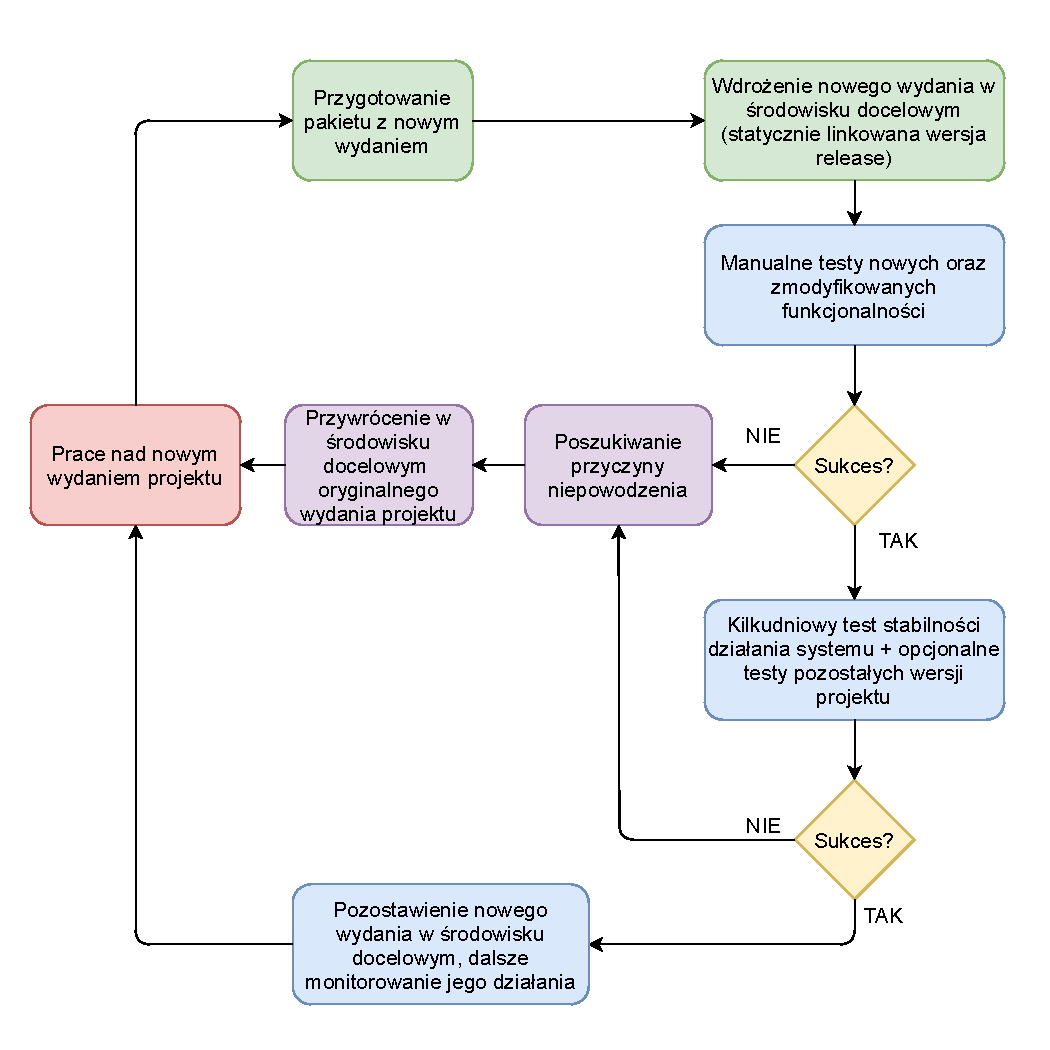
\includegraphics[width=0.85\textwidth]{algorithm.pdf}
\caption{Diagram przedstawiający stosowany przez autorów cykl pracy - kolorem niebieskim oznaczone zostały etapy związane z~regularnymi testami oprogramowania.}
\label{fig:tests_1}
\end{figure}

\section{Testy po migracji systemu (JC)}

Jednym z~ważniejszych etapów pracy magisterskiej była migracja całego systemu GGSS wraz ze sprzętem elektronicznym do nowego środowiska uruchomieniowego. Polegała ona na przeniesieniu kopii oprogramowania na nowy komputer oraz podłączeniu do niego wykorzystywanych urządzeń.

Cała operacja miała odbywać się w~ramach wyjazdu autorów do CERN, natomiast ze względów pandemicznych wyjazd ten został ostatecznie odwołany. Z~tego powodu migracja mogła zostać jedynie częściowo przeprowadzana przez autorów, znaczną część pracy wykonali natomiast eksperci, którzy znajdowali się na miejscu. W~ramach migracji podłączyli oni sprzęt oraz przenieśli zawartość dysków ze starego komputera do nowej maszyny. Przed uruchomieniem całego systemu autorzy zdalnie zweryfikowali poprawność całego procesu. W~ramach tego etapu wykorzystane zostały aplikacje do testowania sprzętu opisane w~sekcji \ref{ch:hardware_testing}. W~trakcie wykonywania testów sprzętu okazało się, że jedynie urządzenie połączone bezpośrednio do komputera jest wykrywane, a~urządzenia połączone za pomocą hub'u USB nie. Rozwiązaniem problemu było podłączenie dodatkowego zasilania wymaganego przez wcześniej wspomniany hub. Upewniwszy się iż sprzęt podłączony jest poprawnie i~jego działanie nie budzi zastrzeżeń, autorzy wykonali sprawdzenia pozostałych elementów środowiska, czyli: zainstalowanych bibliotek, wpisów w~tabeli programu \lstinline{crontab} oraz poprawności umieszczenia plików projektu.

Po sprawdzeniu wszystkich wymaganych elementów środowiska autorzy rozpoczęli proces uruchamiania projektu GGSS wraz z~jego główną aplikacją. W~jego trakcie dokładnie monitorowano zachowanie warstwy oprogramowania oraz urządzeń elektronicznych. Oprócz zachowania aplikacji sprawdzane było również zużycie zasobów oraz ewentualne błędy, które mogły wystąpić ze względu na migrację. Po uruchomieniu projektu monitorowano jego działanie przez kilka godzin, a~następnego dnia dokonano sprawdzenia dziennika zdarzeń. Nie stwierdzono żadnych problemów z~systemem, a~całość działała poprawnie. Migracja została uznana za zakończoną z~sukcesem.

\section{Testy wersji finalnej (AK i~JC)}
Niniejsza sekcja stanowi opis testów finalnej wersji systemu GGSS wykonanych w~sierpniu 2021 roku. Sprawdzeniu poddane zostały zarówno wszystkie najważniejsze funkcjonalności systemu, jak również elementy infrastruktury projektu oraz wprowadzone przez autorów zmiany. Ponadto zbadane zostało zużycie zasobów systemu, takich jak pamięć, podczas długotrwałego, nieprzerwanego działania aplikacji \emph{ggss-runner}. 

\subsection{Testy funkcjonalności głównej aplikacji}
Autorzy dokonali szczegółowego sprawdzenia wszystkich przygotowanych modyfikacji i~rozszerzeń. Ponadto testowane były elementy wchodzące w~skład projektu od początku jego działania. W~kolejnych akapitach opisane zostały poszczególne scenariusze testowe wraz z~otrzymanymi przez autorów wynikami.

\subsubsection*{Działanie komend dedykowanych zasilaczom wysokiego napięcia}
Testom poddana została przygotowana przez autorów składnia komend służących do komunikacji z~zasilaczami wysokiego napięcia. Wykonane zostały sprawdzenia wszystkich trzech typów poleceń (MON, SET, RAW) przy zastosowaniu zróżnicowanych konfiguracji opisujących moduły, kanały oraz parametry. Ze względu na powtarzalny charakter przeprowadzonych sprawdzeń, autorzy zdecydowali się jedynie na przytoczenie wybranych przykładów - wykonane testy obejmowały natomiast wszystkie wspierane parametry komend oraz obsługę wszystkich znanych błędów i~sytuacji wyjątkowych, takich jak niepoprawny format komendy czy typ przekazywanej wartości. Weryfikacja wykonywana była zarówno za pomocą paneli w~środowisku WinCC OA, jak również za pomocą dedykowanego skryptu \lstinline{dimhw.sh}. Listing \ref{lst:test_hw_1} przedstawia przykład testu komendy typu MON, pobierającej wartość oczekiwanego i~monitorowanego napięcia dla wszystkich kanałów każdego z~zasilaczy. Listing \ref{lst:test_hw_2} przedstawia natomiast weryfikację komendy typu SET, zmieniającej wartość napięcia na jednym z~kanałów na wartość 1. Listing \ref{lst:test_hw_3} zawiera przykład wykorzystania komendy typu RAW. Sprawdzenie obsługi sytuacji wyjątkowych zaprezentowane zostało na listingu \ref{lst:test_hw_4}, gdzie do systemu podawana jest niepoprawna nazwa (alias) zasilacza wysokiego napięcia. Testy zakończyły się powodzeniem - wszystkie sprawdzane scenariusze zwróciły wynik zgodny z~oczekiwaniami.

\lstinputlisting[
    language=Cmd, 
    caption={Przykład testu sprawdzającego działanie komendy typu MON, sprawdzającej wartości parametrów VSET i~VMON dla wszystkich kanałów każdego z~zasilaczy.}, 
    label={lst:test_hw_1}
]{6_tests/code_samples/dim_hw_mon.txt}

\lstinputlisting[
    language=Cmd, 
    caption={Przykład testu sprawdzającego działanie komendy typu SET, ustawiającej napięcie na jednym z~kanałów na wartość 1.}, 
    label={lst:test_hw_2}
]{6_tests/code_samples/dim_hw_set.txt}

\lstinputlisting[
    language=Cmd, 
    caption={Przykład testu sprawdzającego działanie komendy typu RAW, sprawdzającej wartość monitorowanego natężenia prądu (parametr IMON) na wybranym kanale.}, 
    label={lst:test_hw_3}
]{6_tests/code_samples/dim_hw_raw.txt}

\lstinputlisting[
    language=Cmd, 
    caption={Przykład testu sprawdzającego zachowanie systemu w~sytuacji, gdy przekazana została niepoprawna nazwa urządzenia.}, 
    label={lst:test_hw_4}
]{6_tests/code_samples/dim_hw_error.txt}

\subsubsection*{Opróżnianie bufora urządzenia MCA}
Sprawdzone zostało poprawne wykonanie algorytmu pozwalającego na zapobieganie przepełnieniu bufora urządzenia MCA poprzez cykliczne przenoszenie jego zawartości do pamięci RAM komputera. Weryfikacji poddane zostały zarówno scenariusze, w~których mechanizm ten nie jest stosowany (np. gdy wartość parametru \lstinline{mcaRefreshInterval} ustawiona została na 0) - wtedy oczekiwanym rezultatem było przepełnienie bufora, jak również te, gdy algorytm był wykorzystywany. Stosowanie przygotowanego rozszerzenia pozwoliło uniknąć błędu przepełnienia bufora, a~zatem umożliwiło pobranie większej ilości danych. Badane były ponadto przypadki specjalne, takie jak wybór większej niż czas pomiaru wartości parametru \lstinline{mcaRefreshInterval} (w tym przypadku system powinien wykonać pobranie danych jedynie przy aktualizacji ELMB w~połowie pomiaru oraz po zakończeniu zbierania danych). Wszystkie testy przyniosły oczekiwane rezultaty, a~zatem przygotowana funkcjonalność działa w~sposób poprawny.

\subsubsection*{Działanie komend sterujących systemem GGSS}
Autorzy poddali testom działanie wszystkich przygotowanych lub zmodyfikowanych komend sterujących systemem GGSS, takich jak: \lstinline{update}, \lstinline{update spectrum} czy też \lstinline{reset channelsOrder}. Ponieważ ich dokładne działanie przedstawione zostało w~części pracy poświęconej przygotowanym ulepszeniom, informacje te nie zostaną tu powtórzone. Podobnie jak w~przypadku pozostałych funkcjonalności, sprawdzane były również przypadki specjalne, takie jak wybór nieistniejącej konfiguracji parametrów początkowych przy dopasowywaniu krzywej do zebranych danych czy też próba przywrócenia oryginalnej kolejności liczników słomkowych, gdy system GGSS nie został zatrzymany. Wszystkie testy zakończyły się zgodne z~przewidywanym zachowaniem systemu. Ponadto sprawdzeniu poddane zostały niektóre z~komend istniejących w~systemie przed modyfikacjami - one również działają poprawnie.

\subsubsection*{Działanie algorytmu dopasowującego krzywą do zebranych danych}
Sprawdzone zostało działanie nowego algorytmu pozwalającego na wyznaczenie parametrów początkowych wykorzystywanych do przeprowadzania dopasowania krzywej do zebranych danych. W~tym przypadku wykonane zostały szczególnie kompleksowe testy, ponieważ przygotowany algorytm ma kluczowy, bezpośredni wpływ na działanie całego systemu. Sprawdzone zostały zatem różne wartości opisujące zakres, w~jakim poszukiwane ma być maksimum lokalne (tzw. \emph{fit range}) - zarówno obejmujące poszukiwany punkt (wtedy oczekiwano sukcesu), jak i~niezawierające go (w takim przypadku oczekiwanym wynikiem był błąd). Ponadto sprawdzone zostały różne wartości parametru \lstinline{smoothingWindowHalf}, odpowiedzialnego za jakość wygładzenia danych za pomocą stosowanego filtru. Szczególnym przypadkiem była tutaj wartość 0~oznaczająca, że algorytm nie powodował zmiany w~danych. Testom poddane zostały ponadto wszystkie cztery konfiguracje parametrów początkowych i~typów dopasowywanej funkcji: \lstinline{GaussFitXe}, \lstinline{GaussFitAr}, \lstinline{Gauss2FitXe} oraz \lstinline{Gauss2FitAr}. Ponadto działanie przygotowanych modyfikacji sprawdzone zostało w~sposób długoterminowy - poprzez monitorowanie poprawności działania systemu w~czasie przeprowadzania testów zużycia zasobów. Autorzy nie wykryli niedoskonałości w~przygotowanym rozwiązaniu, a~zatem uznane zostało ono za poprawne.

\subsubsection*{Pozostałe testy}
Wykonując opisane do tej pory sprawdzenia, autorzy przeprowadzali ponadto szereg testów weryfikujących działanie innych funkcjonalności, zarówno tych modyfikowanych przez nich w~czasie prac nad jakością kodu, jak i~tych niezmienionych. Weryfikacji poddane zostało zatem działanie operacji na plikach i~strukturze XML (odczyt, modyfikacja), tworzenie dziennika zdarzeń czy modyfikowanie kolejności, w~jakiej wykonywany jest pomiar na poszczególnych licznikach słomkowych. Sprawdzane były ponadto funkcjonalności takie jak zerowanie napięć na zasilaczach w~momencie, gdy system kończy swoje działanie. Ponadto, za pomocą istniejących w~ramach infrastruktury WinCC OA paneli przetestowana została możliwość modyfikacji każdego parametru systemu. Przykład panelu pozwalającego na przeprowadzenie tego typu testów przedstawiony został na rysunku \ref{fig:panel-params}. Autorzy dochodzą zatem do wniosku, że z~punktu widzenia oferowanych funkcjonalności system GGSS działa w~pełni poprawnie.

\clearpage
\begin{figure}[H]
    \centering
    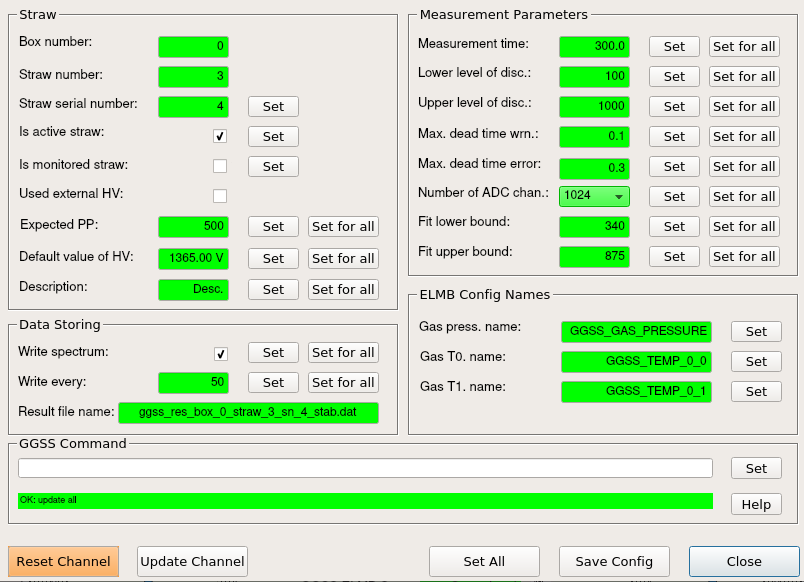
\includegraphics[width=\textwidth]{panel_params.png}
    \caption{Wykorzystany podczas testów panel pozwalający na monitorowanie i~modyfikację parametrów jednego licznika słomkowego.}
    \label{fig:panel-params}
\end{figure}


\subsection{Testy aplikacji oraz skryptów do obsługi urządzeń}

W~ramach testów wersji finalnej przeprowadzono sprawdzenie wszystkich aplikacji do obsługi sprzętu fizycznego, które były modyfikowane, czy też utworzone od zera przez autorów. Testy były przeprowadzane w~środowisku produkcyjnym przy wyłączonym systemie GGSS, a~dokładnie z~wyłączoną główną aplikacją projektu. W~celu sprawdzenia poprawności działania oraz funkcjonalności wykonano zarówno komendy z~użyciem trybu interaktywnego utworzonych aplikacji, jak i~trybu scenariuszowego. W~pierwszej kolejności testom została poddana aplikacja odpowiedzialna za obsługę zasilacza wysokiego napięcia, czyli \emph{high-voltage-service-app}. Listing \ref{lst:high-voltage-service-app-startup} przedstawia wywołanie aplikacji z~wszystkimi wymaganymi argumentami oraz jej wiadomość powitalną. W~ramach tejże wiadomości prezentowane są informację o~utworzeniu połączenia z~modułem zasilacza. Następnie wyświetlana jest informacja o~wykorzystaniu trybu interaktywnego wraz z~krótką pomocą zawierającą format komend.

\clearpage
\lstinputlisting[
    language=Cmd,
    caption={Uruchomienie aplikacji \emph{high-voltage-service-app} w~trybie interaktywnym.},
    label={lst:high-voltage-service-app-startup}
]{6_tests/code_samples/high-voltage-service-app-startup.txt}

Listing \ref{lst:high-voltage-service-app-commands} zawiera przykład działania komend pozwalających na ustawienie wartości napięcia na wyjściu zasilacza, oraz pobrania tejże wartości wraz z~asercją mającą na celu automatyczne sprawdzenie, czy oczekiwana wartość jest zgodna z~rzeczywistą. Trzecie wywołanie komendy ma za zadania sprawdzenie, czy w~przypadku nieotrzymania zadanej wartości aplikacja poprawnie zgłosi błąd. Ostatnie z~wywołań sprawdza poprawność działania asercji z~tolerancją.

\lstinputlisting[
    language=Cmd,
    caption={Komendy wykonywane w~trybie interaktywnym aplikacji \emph{high-voltage-service-app}.},
    label={lst:high-voltage-service-app-commands}
]{6_tests/code_samples/high-voltage-service-app-commands.txt}

Testom poddany został również tryb scenariuszowy, co przedstawia listing \ref{lst:high-voltage-service-app-scenario}. W~tym przypadku najpierw wyświetlane są informacje o~komendach przetworzonych w~ramach danego pliku scenariuszowego, a~dopiero później następuje ich uruchomienie, zgodnie ze specyfikacją zawartą w~argumentach wywołania aplikacji.

\lstinputlisting[
    language=Cmd,
    caption={Przykładowe uruchomienie aplikacji \emph{high-voltage-service-app} w~trybie scenariuszowym. Zawartość scenariusza została skrócona na potrzeby manuskryptu.},
    label={lst:high-voltage-service-app-scenario}
]{6_tests/code_samples/high-voltage-service-app-scenario.txt}

Wszystkie testy aplikacji \emph{high-voltage-service-app} przebiegły pomyślne. Aplikacja wykonała wszystkie żądane czynności, a~odpowiednie wartości pojawiły się na zasilaczu wysokiego napięcia. Zarówno tryb interaktywny, jak i~scenariuszowy zostały uruchomione bez problemu. Aplikacja zachowywała się poprawnie również w~przypadku, gdy oczekiwane było zgłoszenie błędu.

Następnie w~podobny sposób przetestowane zostało dzianie aplikacji \emph{multiplexer-service-app}. Przetestowano zarówno jej tryb interaktywny, jak i~scenariuszowy. Ze względu na to, że testy wyglądały analogicznie jak w~przypadku aplikacji \emph{high-voltage-service-app}, a~różnice stanowiły jedynie komendy oraz odpowiedzi od urządzenia, zaprezentowany został jedynie listing \ref{lst:multiplexer-service-app}, który przedstawia wiadomość powitalną aplikacji do obsługi multipleksera oraz kilka podstawowych komend.

\clearpage
\lstinputlisting[
    language=Cmd,
    caption={Przykład działania aplikacji \emph{multiplexer-service-app} - przedstawiona została wiadomość powitalna zawierająca informacje na temat możliwości aplikacji oraz wykonanie kilku przykładowych komend, powodujących pobranie numeru seryjnego urządzenia oraz pobranie i~zmianę aktywnego kanału.},
    label={lst:multiplexer-service-app}
]{6_tests/code_samples/multiplexer-service-app.txt}

W~przypadku aplikacji \emph{multiplexer-service-app} wszystkie testy udało się przeprowadzić pomyślnie. Nie stwierdzono żadnych błędów w~działaniu wyżej wymienionej aplikacji. Wszystkie funkcjonalności, tryb interaktywny, jak i~tryb scenariuszowy działały poprawnie.

\clearpage
Testy aplikacji \emph{high-voltage-killer} oraz skryptów składających się na system awaryjnego wyłączania wysokiego napięcia polegały zarówno na uruchomieniu samego programu i~sprawdzeniu, czy jego działanie jest poprawne oraz na symulowaniu rzeczywistych warunków, w~ramach których program powinien zostać uruchomiony. 

W~pierwszej kolejności wykorzystano wcześniej przetestowaną aplikację \emph{high-voltage-service-app} w~celu ustawienia napięcia na zasilaczu wysokiego napięcia na wartość większą niż zero, następnie uruchomiono aplikację \emph{high-voltage-killer}, co przedstawia listing \ref{lst:high-voltage-killer}. W~ramach działania aplikacja analizuje znajdujące się w~systemie pliki urządzeń, następnie wybiera te, za pomocą których podłączone są zasilacze wysokiego napięcia. Następnie, wykorzystując bibliotekę \emph{caenn1470-lib}, zerowane są napięcia na wszystkich wyjściach wszystkich podłączonych modułów. Aplikacja prewencyjne próbuje zerować napięcia na modułach od 0~do 7, nawet, gdy tylko 3~moduły są uruchomione, natomiast komendy wysyłane są jedynie do podłączonych modułów.

\lstinputlisting[
    language=Cmd,
    caption={Uruchomienie aplikacji \emph{high-voltage-killer}},
    label={lst:high-voltage-killer}
]{6_tests/code_samples/high-voltage-killer.txt}

Następnie ponownie wykorzystując aplikację \emph{high-voltage-service-app} sprawdzono, czy rzeczywiście napięcie zostało wyzerowane. Wykonując odpowiednie komendy stwierdzono, że test przebiegł pomyślnie. Oprócz samego działania aplikacji \emph{high-voltage-killer} przetestowano również funkcjonalności dostarczane w~skryptach współpracujących z~tą aplikacją:
\begin{itemize}
    \item Uruchomienie aplikacji \emph{high-voltage-killer} jeżeli główna aplikacja GGSS przestała działać i~nie została uruchomiona w~przeciągu 5~minut
    \item Możliwość zablokowania systemu awaryjnego wyłączania zasilania poprzez utworzenie pliku blokady.
    \item Ciągłe działanie systemu awaryjnego wyłączania zasilania w~przypadku braku pliku blokady.
    \item Awaryjne wyłączenie zasilania w~przypadku otrzymania sygnału SIGTERM
\end{itemize}

Przeprowadzone testy wszystkich wyżej wymienionych funkcjonalności przebiegły pomyślnie. Nie napotkano żadnych przeszkód w~trakcie ich wykonywania. Dodatkowo przeprowadzono testy aplikacji \emph{device-detector}, której zadaniem jest raportowanie informacji o~podłączonych do systemu urządzeniach, które wymagane są do działania systemu GGSS. Również w~tym przypadku proces przebiegł pomyślne. W~celu osiągnięcia pewności, iż wszystkie aplikacje związane ze sprzętem fizycznym działają poprawnie w~nowym środowisku testom została poddana również aplikacja \emph{mca-service-app}. Uruchomienie tejże aplikacji nie spowodowało żadnych problemów, a~wyniki jej działania były poprawne. Wraz z~zakończeniem tego testu wszystkie aplikacje oraz skrypty związane ze sprzętem zostały w~pełni przetestowane, dzięki czemu autorzy mogli być pewni poprawności zaimplementowanych funkcjonalności.


\subsection{Testy wykorzystania pamięci operacyjnej}

Zwieńczeniem testów, które miało zapewnić długotrwałe, bezproblemowe działanie projektu GGSS, było monitorowanie, przez długi okres czasu, zasobów systemowych przypisanych do głównej aplikacji. W~tym celu wykorzystano wcześniej opisany skrypt \lstinline{check_resource_usage_ggss.sh}. Najważniejszym monitorowanym parametrem był RSS (\emph{Resident Set Size}), który przedstawiał ilość pamięci RAM wykorzystywanej przez proces. Ze względu na to, że aplikacja \emph{ggss-runner} powinna działać bez zakłóceń przez okres co najmniej kilku miesięcy ważne było, aby test wykazał brak zwiększającego się zużycia pamięci, mogącego w~dłuższym okresie czasu doprowadzić do wyczerpania jej zasobów w~systemie.

Rysunek \ref{fig:rss-short} przedstawia ilość wykorzystywanej pamięci (RSS) względem czasu. Na rysunku przedstawiony został okres od dnia 10 sierpnia 2021 roku w~południe do końca dnia 11 sierpnia 2021 roku. W~trakcie tego okresu autorzy przeprowadzali testy z~wykorzystaniem platformy Valgrind, co widoczne jest na wykresie w~okresach, w~których zużycie pamięci znacząco odstaje od normy, która plasuje się w~okolicach 6000 kB. Dnia 10 sierpnia 2021 roku autorzy wykonywali testy z~wykorzystaniem narzędzia Massif - w~trakcie korzystania z~tego narzędzia zużycie pamięci wynosiło niecałe 50 tysięcy kB. W~przypadku odstępstwa z~dnia 11 sierpnia wykorzystane zostało narzędzie Memcheck, a~zużycie pamięci wyniosło znacznie powyżej 200 tysięcy kB. Na wykresie widoczny jest również charakterystyczny ogon związany z~ponownym uruchomieniem aplikacji. Wynika on z~faktu, iż aplikacja w~fazie inicjalizacji oraz w~trakcie początkowych pomiarów alokuje pamięć na wszystkie potrzebne zmienne wraz z~buforami na przechowywanie danych pozyskanych z~urządzeń fizycznych wchodzących w~skład systemu GGSS.

\clearpage
\begin{figure}[H]
    \centering
    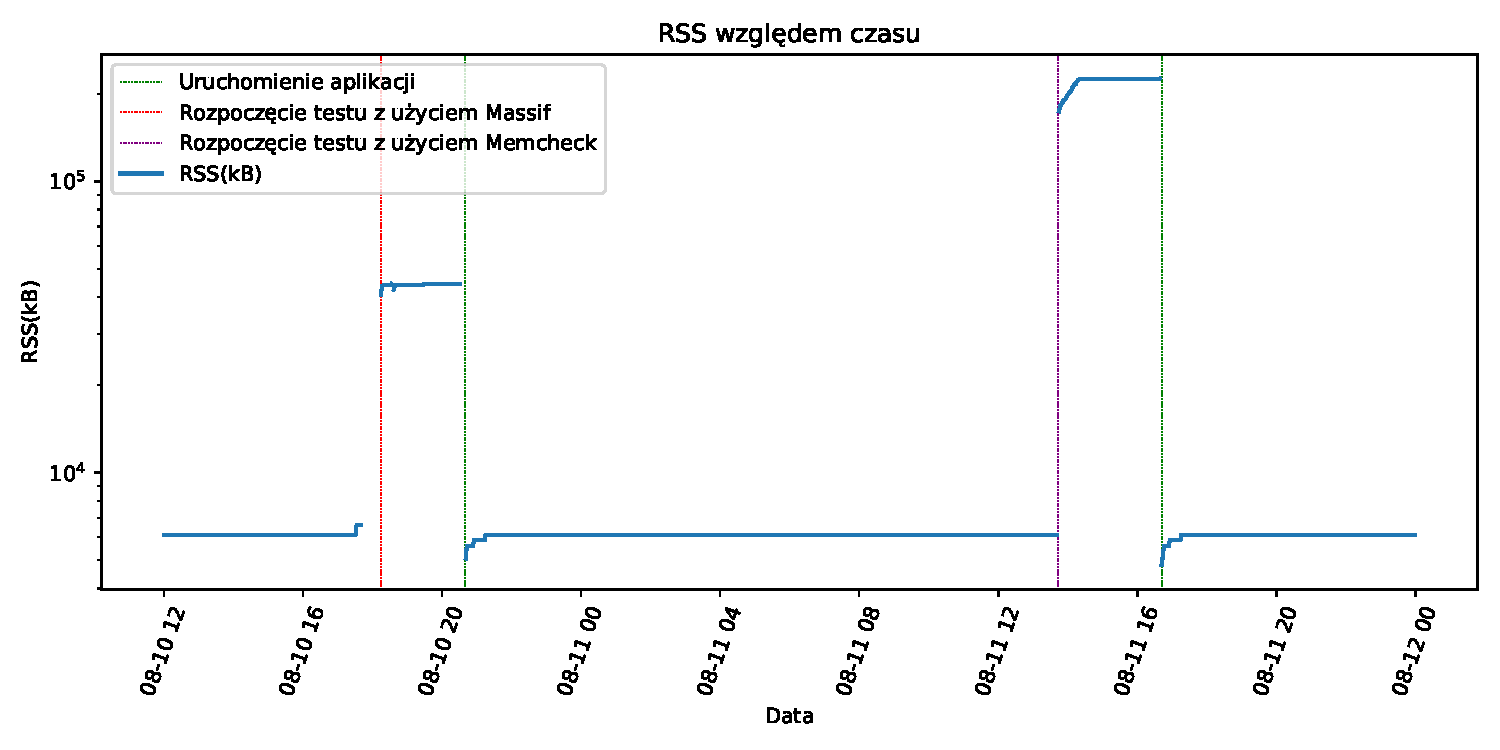
\includegraphics[width=0.9\textwidth]{rss_short.pdf}
    \caption{Wykres przedstawiający zużycie pamięci (RSS) przez aplikację \emph{ggss-runner} względem czasu w~okresie od 10 sierpnia 2021 roku do końca 11 sierpnia 2021 roku.}
    \label{fig:rss-short}
\end{figure}

W~celu dokładniejszej weryfikacji długotrwałego zużycia pamięci przygotowany został również rysunek \ref{fig:rss-long}. Przedstawia on parametr RSS względem czasu dla dłuższego okresu monitorowania. Oprócz charakterystycznych odstępstw od normy związanych z~wykorzystaniem platformy Valgrind nie zaobserwowano żadnych anomalii. Zmiany ilości wykorzystywanej pamięci wiązały się jedynie z~początkową inicjalizacją zmiennych, buforów na dane, czy też wynikały z~interakcji z~systemem, np.: poprzez wysłanie do niego komend. W~przypadku, gdy aplikacja \emph{ggss-runner} działała bez zewnętrznych poleceń, czy też zakłóceń, to zużycie pamięci nie zwiększało się przez dłuższy okres czasu.

\begin{figure}[H]
    \centering
    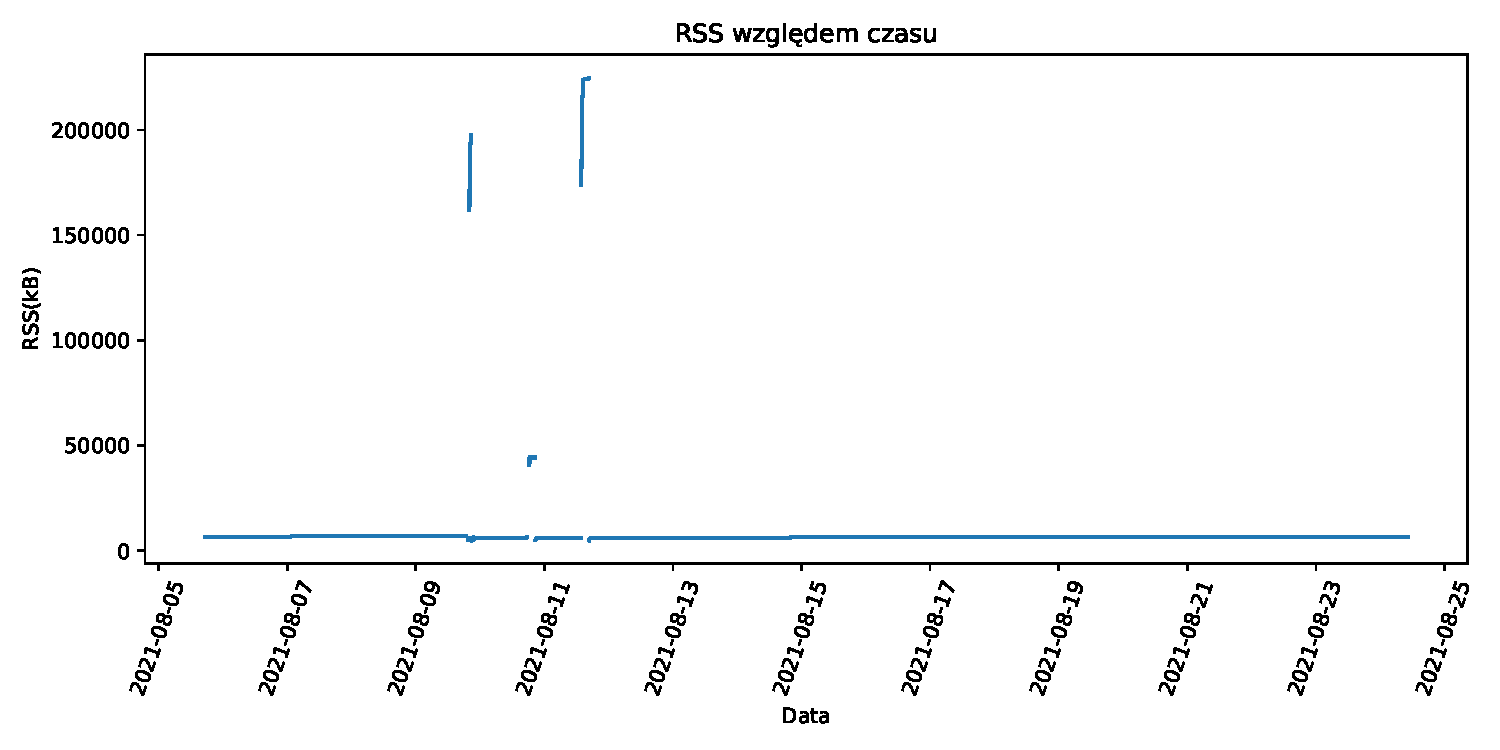
\includegraphics[width=0.9\textwidth]{rss_long.pdf}
    \caption{Wykres przedstawiający zużycie pamięci (RSS) przez aplikację \emph{ggss-runner} względem czasu w~okresie od 5~sierpnia 2021 roku do 25 sierpnia 2021 roku.}
    \label{fig:rss-long}
\end{figure}

W~celu zbadania występowania potencjalnych błędów w~zarządzaniu wykorzystania pamięcią użyto narzędzie Memcheck wchodzące w~skład platformy Valgrind. Testy wykazały obecność nieprawidłowości, jednakże wygenerowany raport wskazuje, że pochodzą one z~bibliotek zewnętrznych wykorzystywanych w~projekcie, w~tym przede wszystkim z~biblioteki DIM oraz Boost.Log. Na listingu \ref{lst:memcheck-error} umieszczony został fragment raportu z~działania narzędzia Memcheck prezentujący przykładowy błąd związany z~faktem, że biblioteka DIM nie dokonuje poprawnego zwolnienia alokowanej pamięci. Po analizie wszystkich zgłoszonych przez narzędzie błędów, autorzy stwierdzili, że żaden z~nich nie powoduje stopniowego wzrostu wykorzystywanej pamięci operacyjnej. Na tej podstawie zostało stwierdzone, że nie zagrażają one bezpieczeństwu długotrwałego działania aplikacji.

\lstinputlisting[
    language=Cmd,
    caption={Przykładowy, powodowany przez bibliotekę DIM, błąd raportowany przez narzędzie Memcheck.},
    label={lst:memcheck-error}
]{6_tests/code_samples/memcheck-error.txt}

Dodatkowym argumentem przemawiającym za poprawnością wyżej przytoczonych wniosków jest fakt, iż niezależnie od długości przeprowadzanego testu z~użyciem narzędzia Memcheck rozmiar pamięci oznaczonej jako \lstinline{still reachable} pozostawał niezmienny i~wynosił ok 178kB, co zostało zaprezentowane na listingu \ref{lst:memcheck-leak-summary}.

\lstinputlisting[
    language=Cmd,
    caption={Podsumowanie wycieków pamięci raportowane przez narzędzie Memcheck.},
    label={lst:memcheck-leak-summary}
]{6_tests/code_samples/memcheck-leak-summary.txt}

Przeprowadzone zostały również, trwające nieco poniżej dwóch godzin, testy zużycia pamięci sterty i~stosu z~wykorzystaniem narzędzia Massif wchodzącym w~skład platformy Valgrind. Wynik zaprezentowany został na rysunku \ref{fig:massif-long}. W~początkowym etapie testu widoczne jest stopniowe wzrastanie zużycia pamięci. Wynika ono z~przeprowadzania pierwszych iteracji pomiarów na wszystkich licznikach słomkowych podczas których alokowana jest pamięć pozwalająca na przechowywanie wyników z~ostatnich kilku iteracji dla danego licznika. Następnie zużycie pamięci pozostaje stałe, aż do momentu rozpoczęcia procesu zakańczania działania programu, gdy rośnie ono na krótką chwilę. Przeprowadzony test dowodzi, że w~czasie regularnego działania systemu zużycie pamięci pozostaje stałe.

\begin{figure}[H]
    \centering
    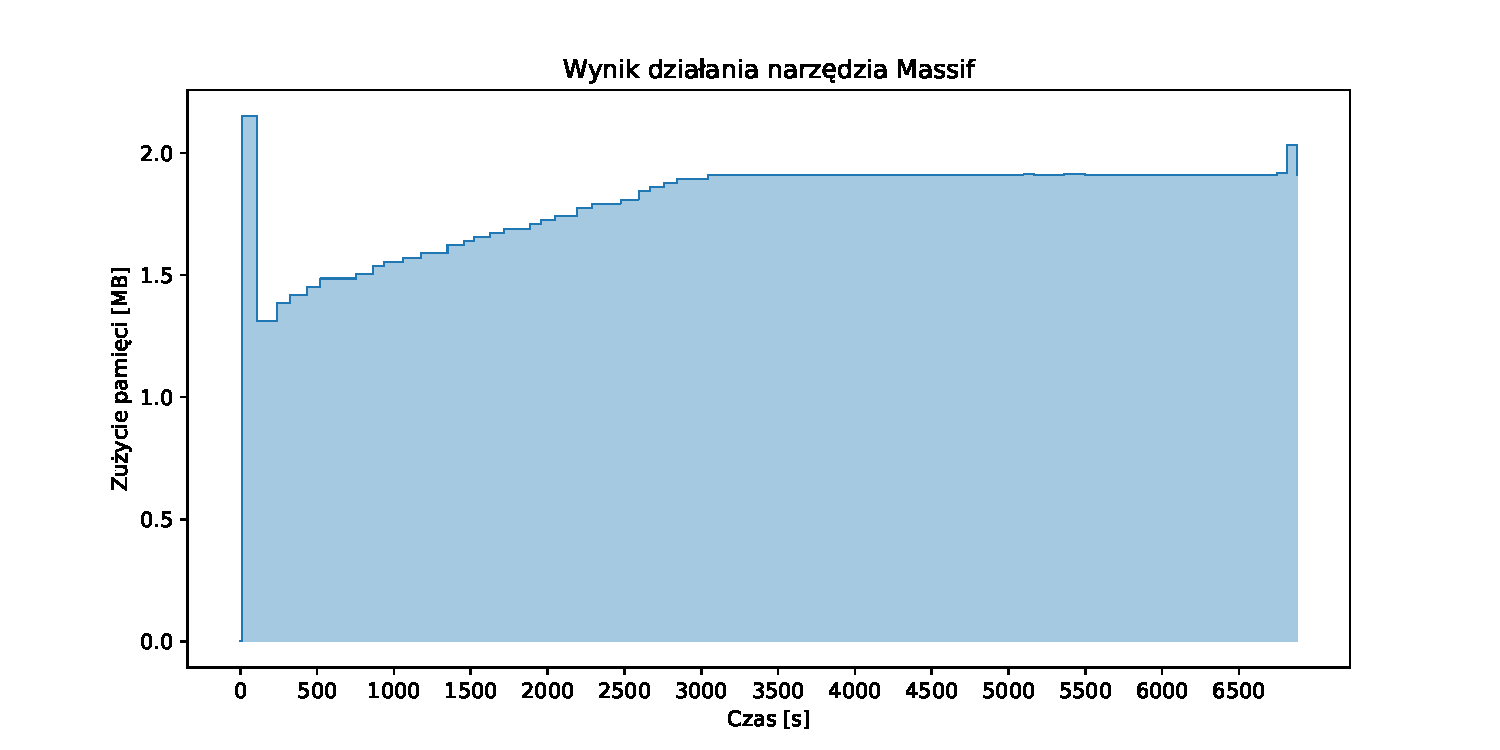
\includegraphics[width=\textwidth]{massif_plot_long.pdf}
    \caption{Wykres przedstawiający zużycie pamięci sterty i~stosu zbadane z~wykorzystaniem narzędzia Massif.}
    \label{fig:massif-long}
\end{figure}

Przeprowadzone przez autorów testy wskazują na stabilne zachowanie programu pod kątem zużywanych zasobów systemowych, m.in. pamięci operacyjnej. Przeprowadzone zostały ponadto testy wykorzystania czasu procesora, które również wskazują na stabilne działanie programu.
